\documentclass[titlepage]{article}

\usepackage[dutch]{babel}
\usepackage{fancyhdr}
\usepackage[margin=2cm]{geometry}
\usepackage{graphicx}
\usepackage[utf8]{inputenc}
\usepackage{siunitx}
\usepackage{tikz}

\usetikzlibrary{arrows}

\graphicspath{{schermafdrukken/}}

\sisetup{detect-weight=true, detect-family=true}

\title{
    Practicum 3: \\
    \large{Communicerende automaten}
}

\author{
    Caro Meysmans \\
    \texttt{Caro.Meysmans@UGent.be}
    \and
    Lukas De Loose \\
    \texttt{Lukas.DeLoose@UGent.be}
    \and
    Garben Tanghe \\
    \texttt{Garben.Tanghe@UGent.be}
}

\pagestyle{fancy}

% Clear header and footer
\fancyhf{}

\lhead{Practicum 3}
\rhead{Communicerende automaten}
\lfoot{Groep 11}
\rfoot{Pagina \thepage}

\newcommand{\question}[1]{\noindent \textbf{#1} \\}

\begin{document}

\maketitle

\tableofcontents
\listoffigures

\clearpage

\section{De woordgenerator}

De woordgenerator implementeren we als een synchrone automaat met 13 toestanden.
De resettoestand zet de uitgangsbits op \texttt{"0000"}.
De reset is asynchroon.
De overige 12 toestanden zetten de gewenste sequentie op de uitgangsbits.
We bemerken dat wanneer de \texttt{enable}-ingang laag staat,
er geen nieuw woord naar buiten wordt gebracht.

\begin{figure}[htpb]
    \centering
    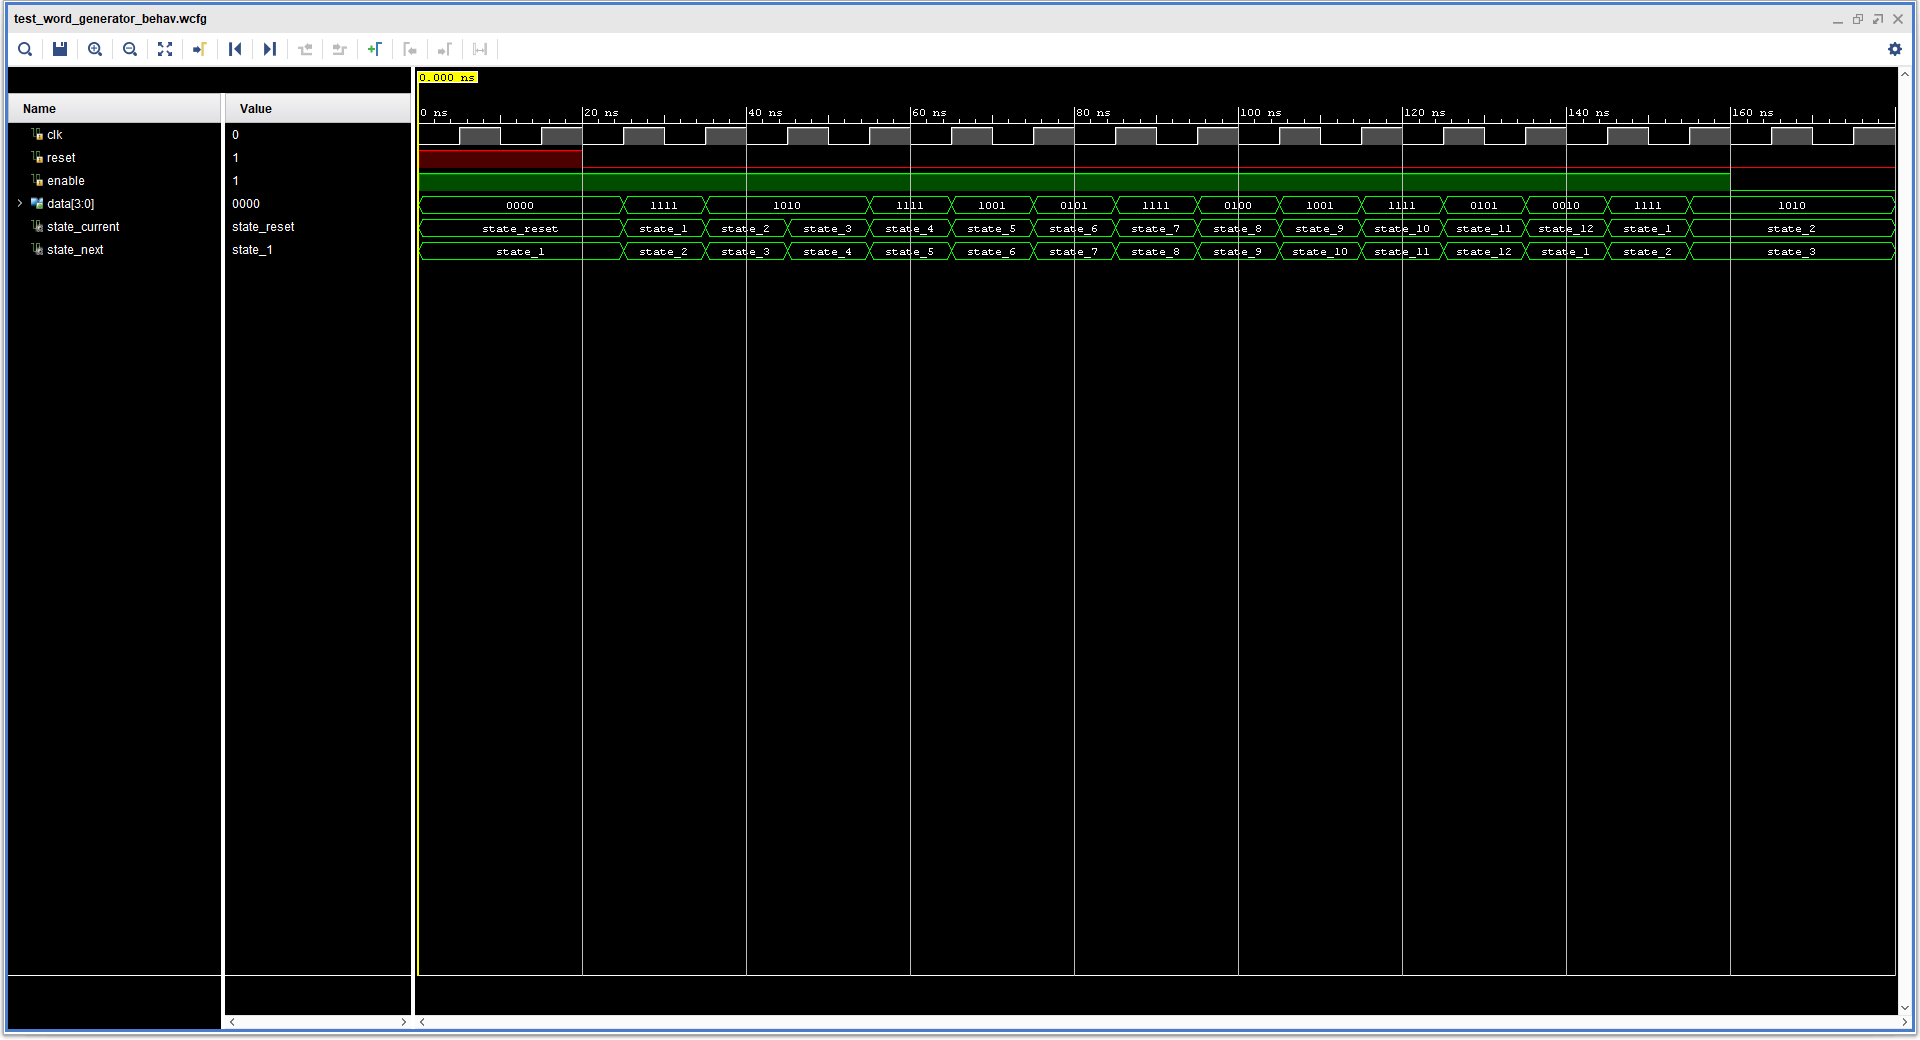
\includegraphics[trim={0 500px 0 0}, clip, width =\linewidth]{word_generator_gedragssimulatie.PNG}
    \caption{\texttt{word\_generator} gedragssimulatie}
    \label{fig:word_generator_behav}
\end{figure}

\section{De eerste zender en ontvanger}

\begin{figure}[h!]
    \centering
    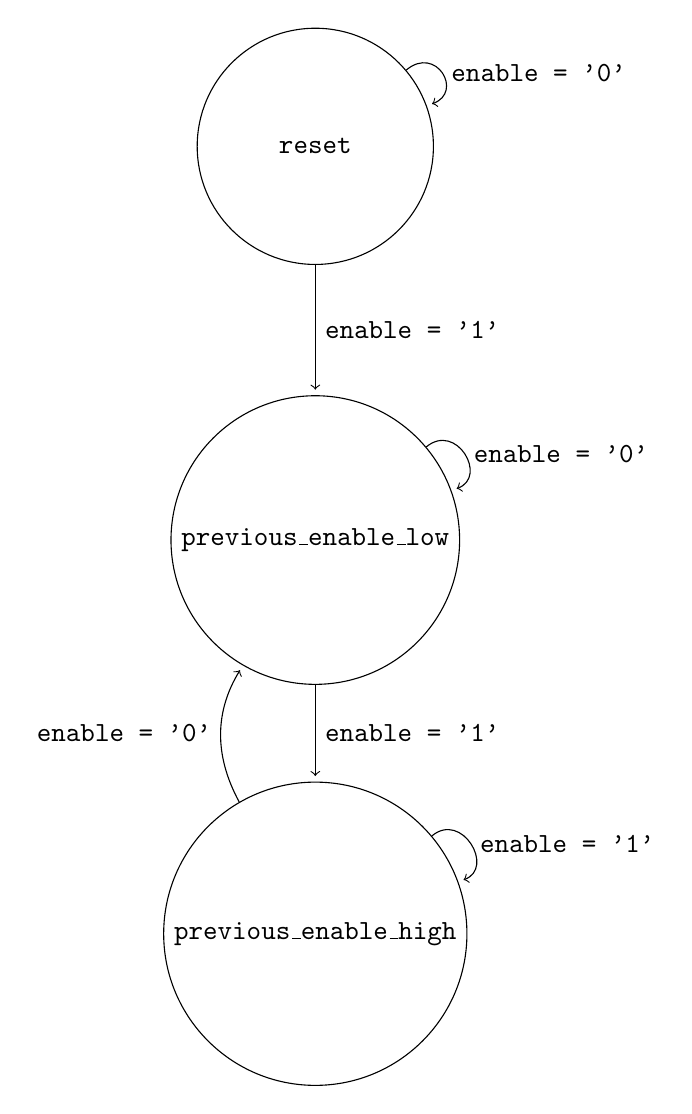
\begin{tikzpicture}[
        shorten >= 2 pt,
        state/.style = {
            draw, circle,
            align=center,
            minimum width = 3cm,
            node distance = 5cm,
        },
        ]

        % Toestanden
        \node[state] (reset) {\texttt{reset}};
        \node[state, below of = reset] (previous_enable_low) {\texttt{previous\_enable\_low}};
        \node[state, below of = previous_enable_low] (previous_enable_high) {\texttt{previous\_enable\_high}};


        % Transities
        \path
            [
            ->,
            every loop/.style = {
                in = 20,
                out = 40,
                looseness = 0
            }
            ]
            (reset) edge[loop] node[right] {\texttt{enable = '0'}} (reset)
            (previous_enable_low) edge[loop] node[right] {\texttt{enable = '0'}} (previous_enable_low)
            (previous_enable_high) edge[loop] node[right] {\texttt{enable = '1'}} (previous_enable_high);

        \path
            [
            ->
            ]
            (reset) edge node[right] {\texttt{enable = '1'}} (previous_enable_low)
            (previous_enable_low) edge node[right] {\texttt{enable = '1'}} (previous_enable_high)
            (previous_enable_high) edge [bend left] node[left] {\texttt{enable = '0'}} (previous_enable_low);
    \end{tikzpicture}

    \caption{\texttt{r1} toestandstransitiediagram}
    \label{fig:r1_toestandstransitiediagram}
\end{figure}

\noindent \textbf{Wanneer verwacht je dat het mis zal lopen? Toon aan met simulaties dat je verwachtingen kloppen.} \\
Daar de klokperiodes van zender en ontvanger gelijk zijn,
verwachten we dat het mis zal lopen als \texttt{delay2} groter wordt dan de klokperiode van de ontvanger.
In deze situatie is het woord aan de ingang van de ontvanger niet op tijd stabiel.
De volgende gedragssimulaties staven onze verwachtingen.

Nu laten we de zender op een kloksignaal van \SI{10}{\nano\second} lopen.
Indien we vervolgens de ontvanger op een kloksignaal van \SI{7}{\nano\second} en \SI{13}{\nano\second} laten lopen,
bemerken we dat de automaten niet meer succesvol communiceren.
Het verschil in klokperiodes zorgt dat beiden woordgeneratoren niet synchroon lopen.
In de eerste situatie zal de ontvanger meermaals hetzelfde woord inlezen, aangezien de zender niet tijdig een nieuw woord kan genereren.
In de tweede situatie zal de ontvanger woorden overslaan, aangezien deze niet tijdig klaar is om een nieuw woord in te lezen.

\begin{figure}[htpb]
    \centering
    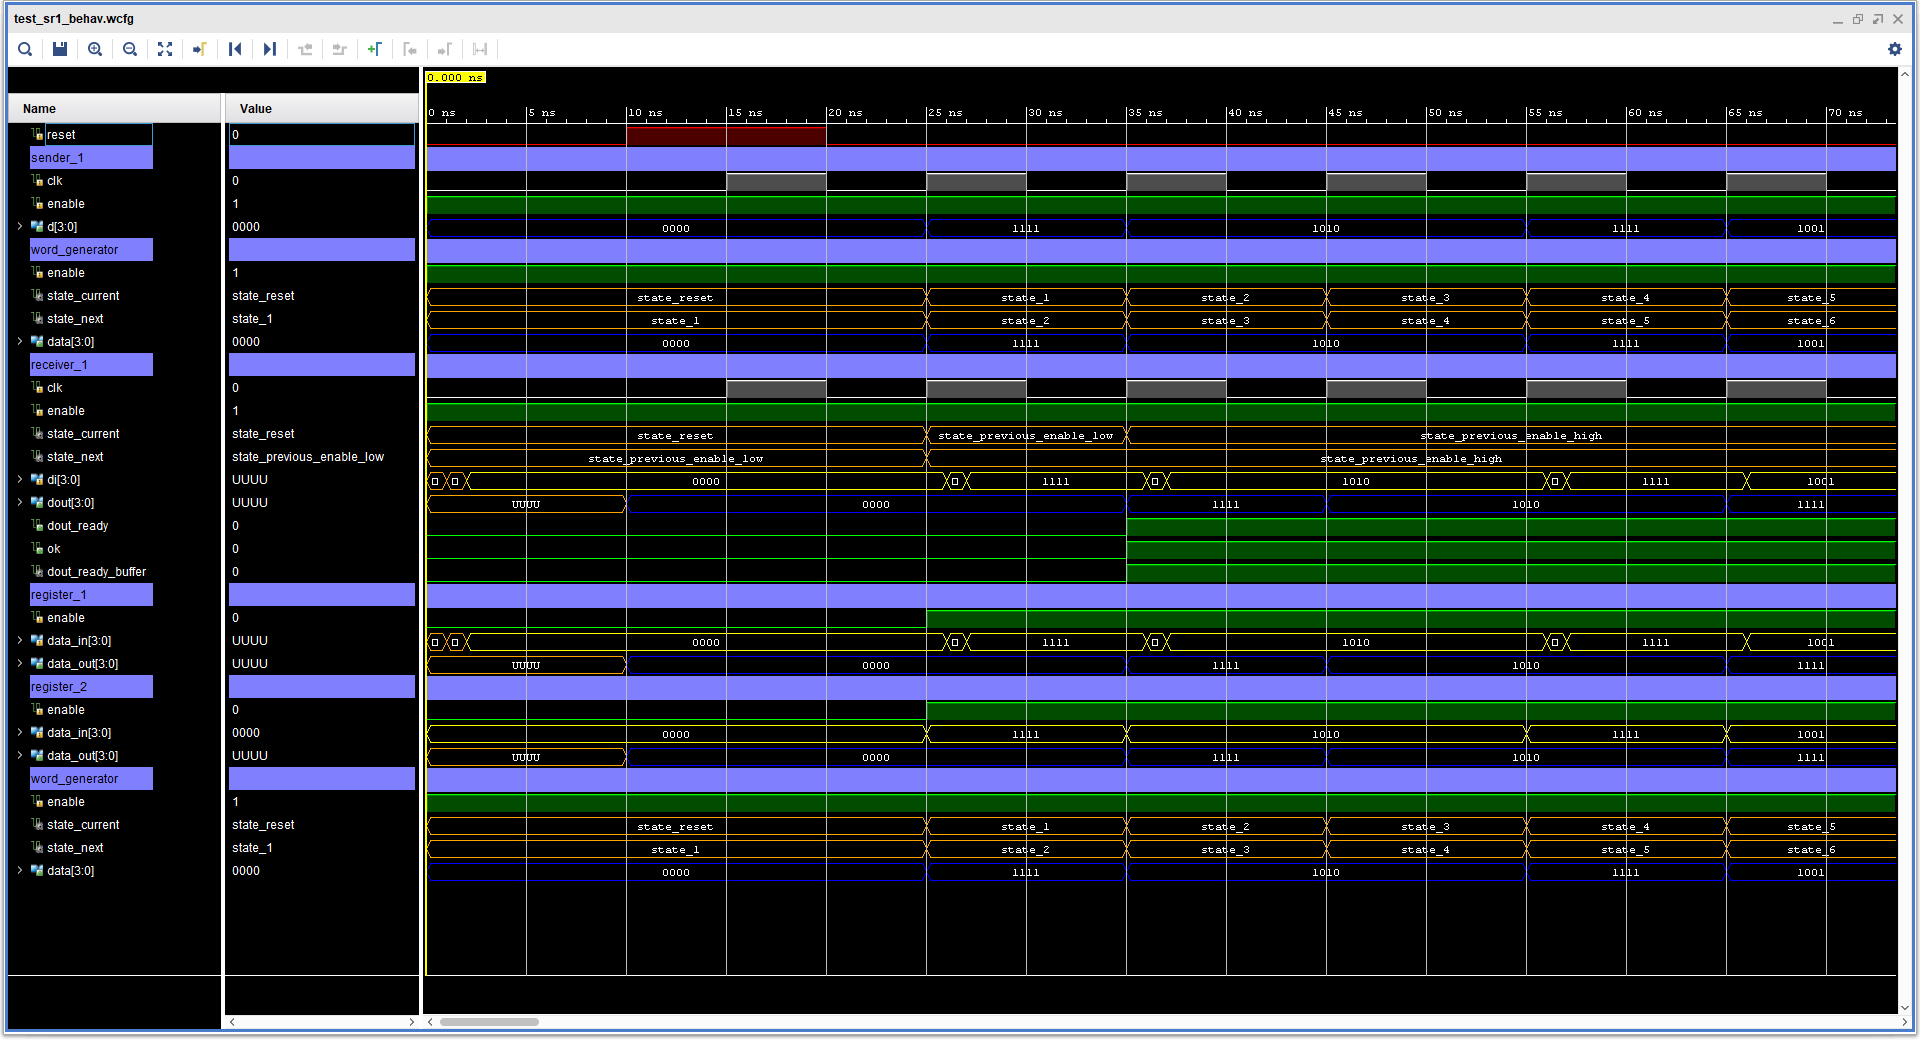
\includegraphics[trim={0 100px 0 0}, clip, width =\linewidth]{sr1_gedragssimulatie_10_10_1_2.PNG}
    \caption{\texttt{s\_1}, \texttt{r\_1} gedragssimulatie bij \(T_1 = \SI{10}{\nano\second}, T_2 = \SI{10}{\nano\second}, \Delta_1 = \SI{1}{\nano\second}, \Delta_2 = \SI{2}{\nano\second} \)}
    \label{fig:sr1_behav_10_10_1_2}
\end{figure}

\begin{figure}[htpb]
    \centering
    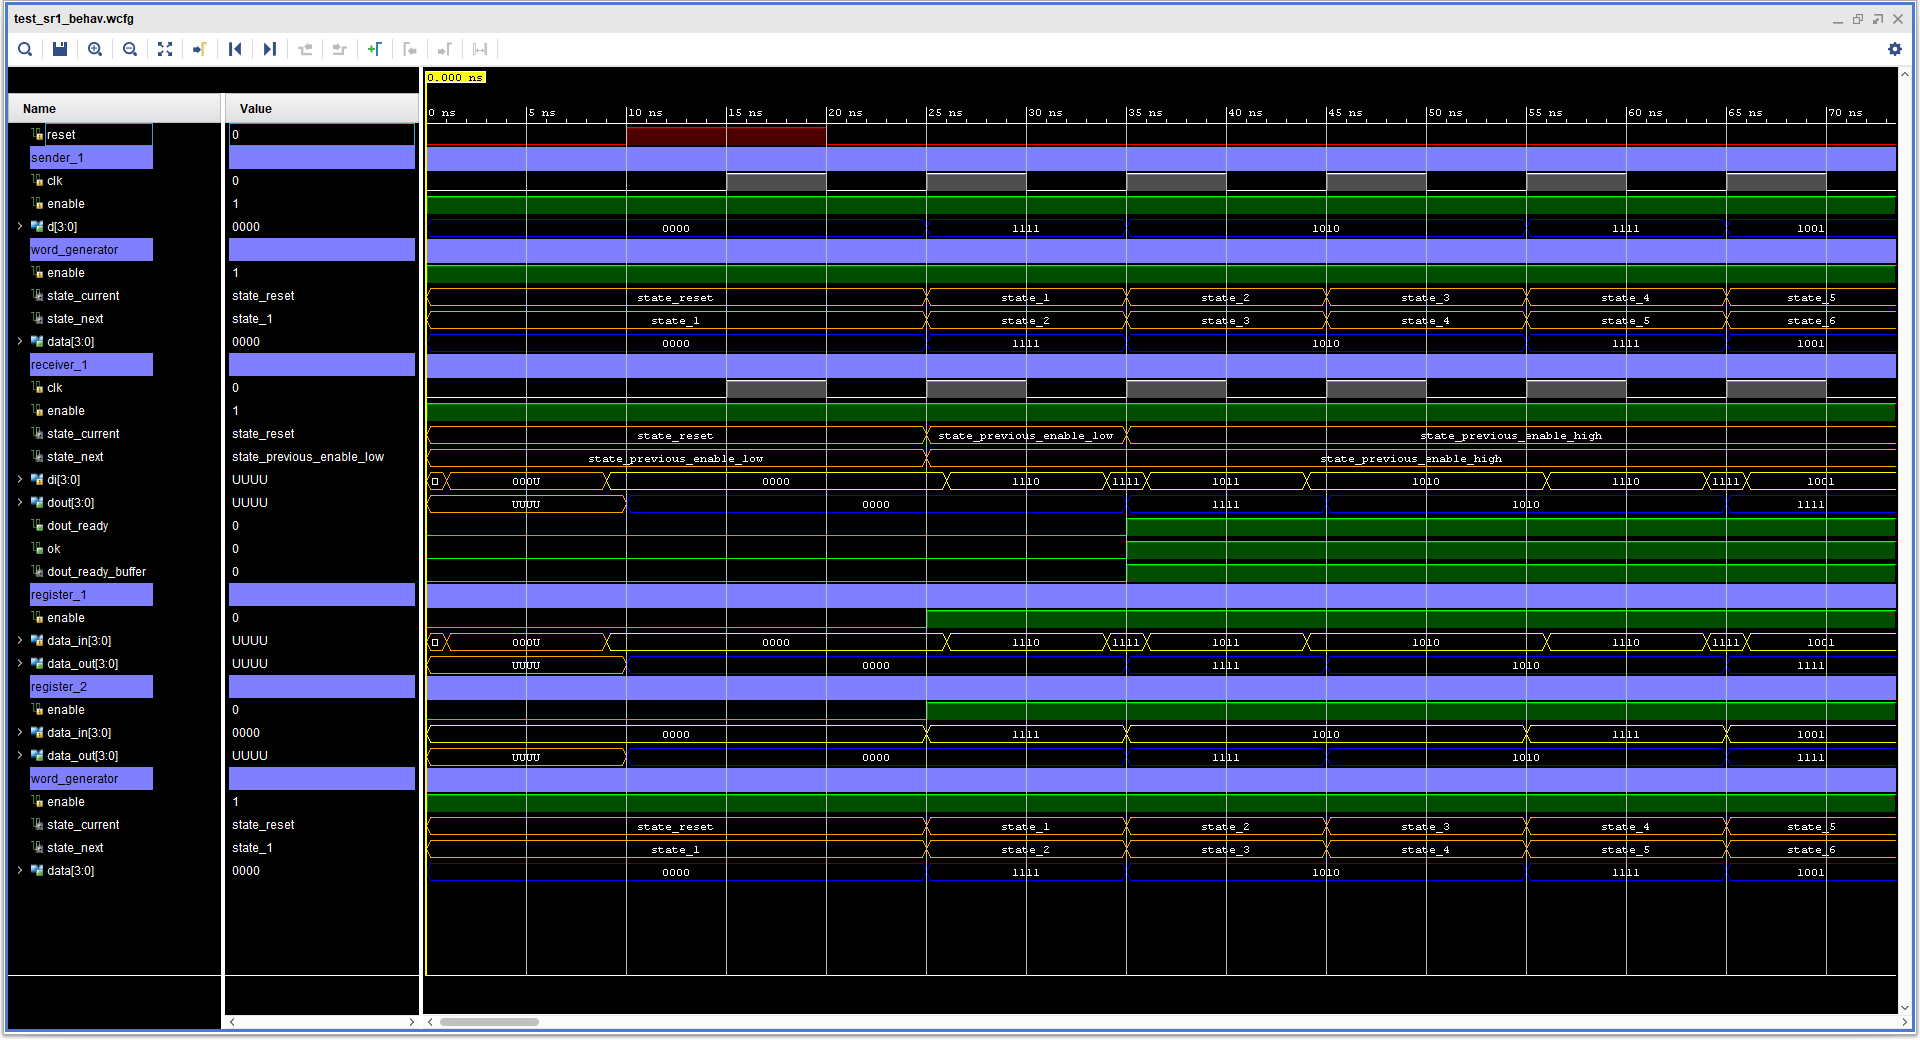
\includegraphics[trim={0 100px 0 0}, clip, width =\linewidth]{sr1_gedragssimulatie_10_10_1_9.PNG}
    \caption{\texttt{s\_1}, \texttt{r\_1} gedragssimulatie bij \(T_1 = \SI{10}{\nano\second}, T_2 = \SI{10}{\nano\second}, \Delta_1 = \SI{1}{\nano\second}, \Delta_2 = \SI{9}{\nano\second} \)}
    \label{fig:sr1_behav_10_10_1_9}
\end{figure}

\begin{figure}[htpb]
    \centering
    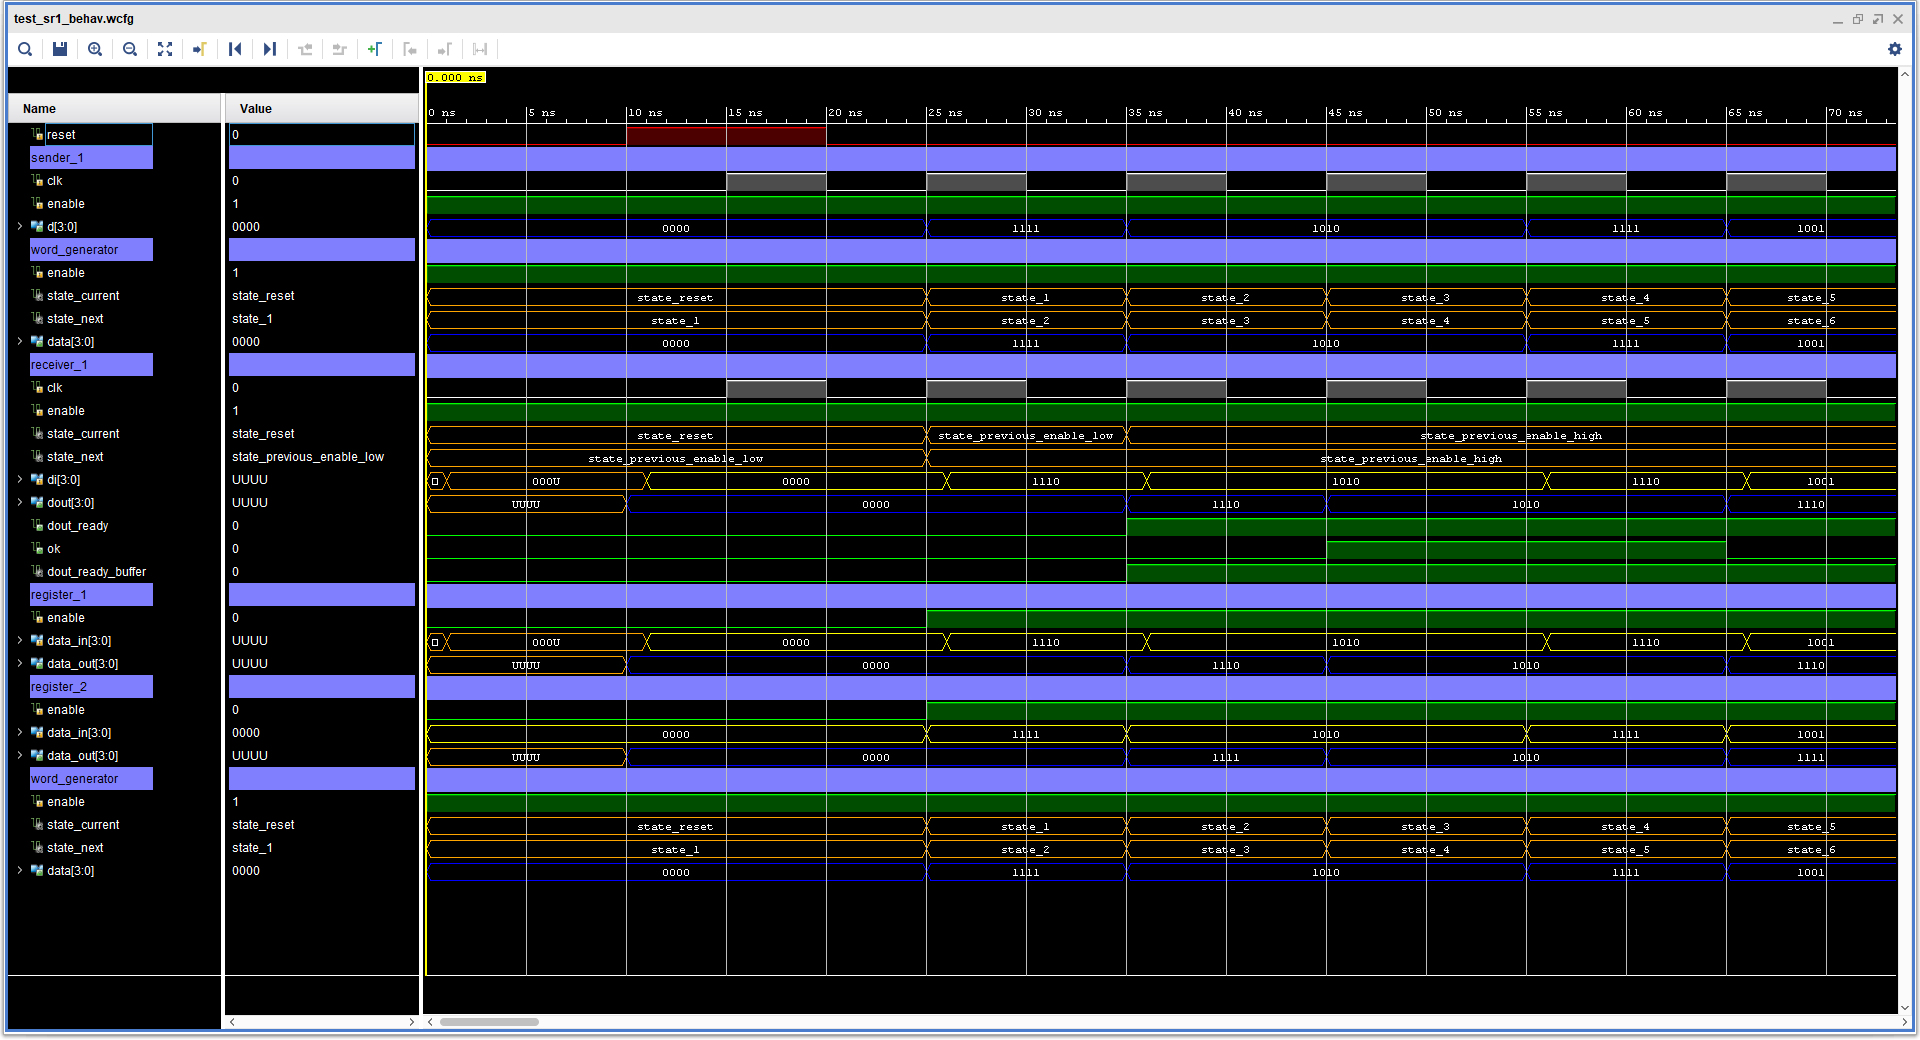
\includegraphics[trim={0 100px 0 0}, clip, width =\linewidth]{sr1_gedragssimulatie_10_10_1_11.PNG}
    \caption{\texttt{s\_1}, \texttt{r\_1} gedragssimulatie bij \(T_1 = \SI{10}{\nano\second}, T_2 = \SI{10}{\nano\second}, \Delta_1 = \SI{1}{\nano\second}, \Delta_2 = \SI{11}{\nano\second} \)}
    \label{fig:sr1_behav_10_10_1_11}
\end{figure}

\begin{figure}[htpb]
    \centering
    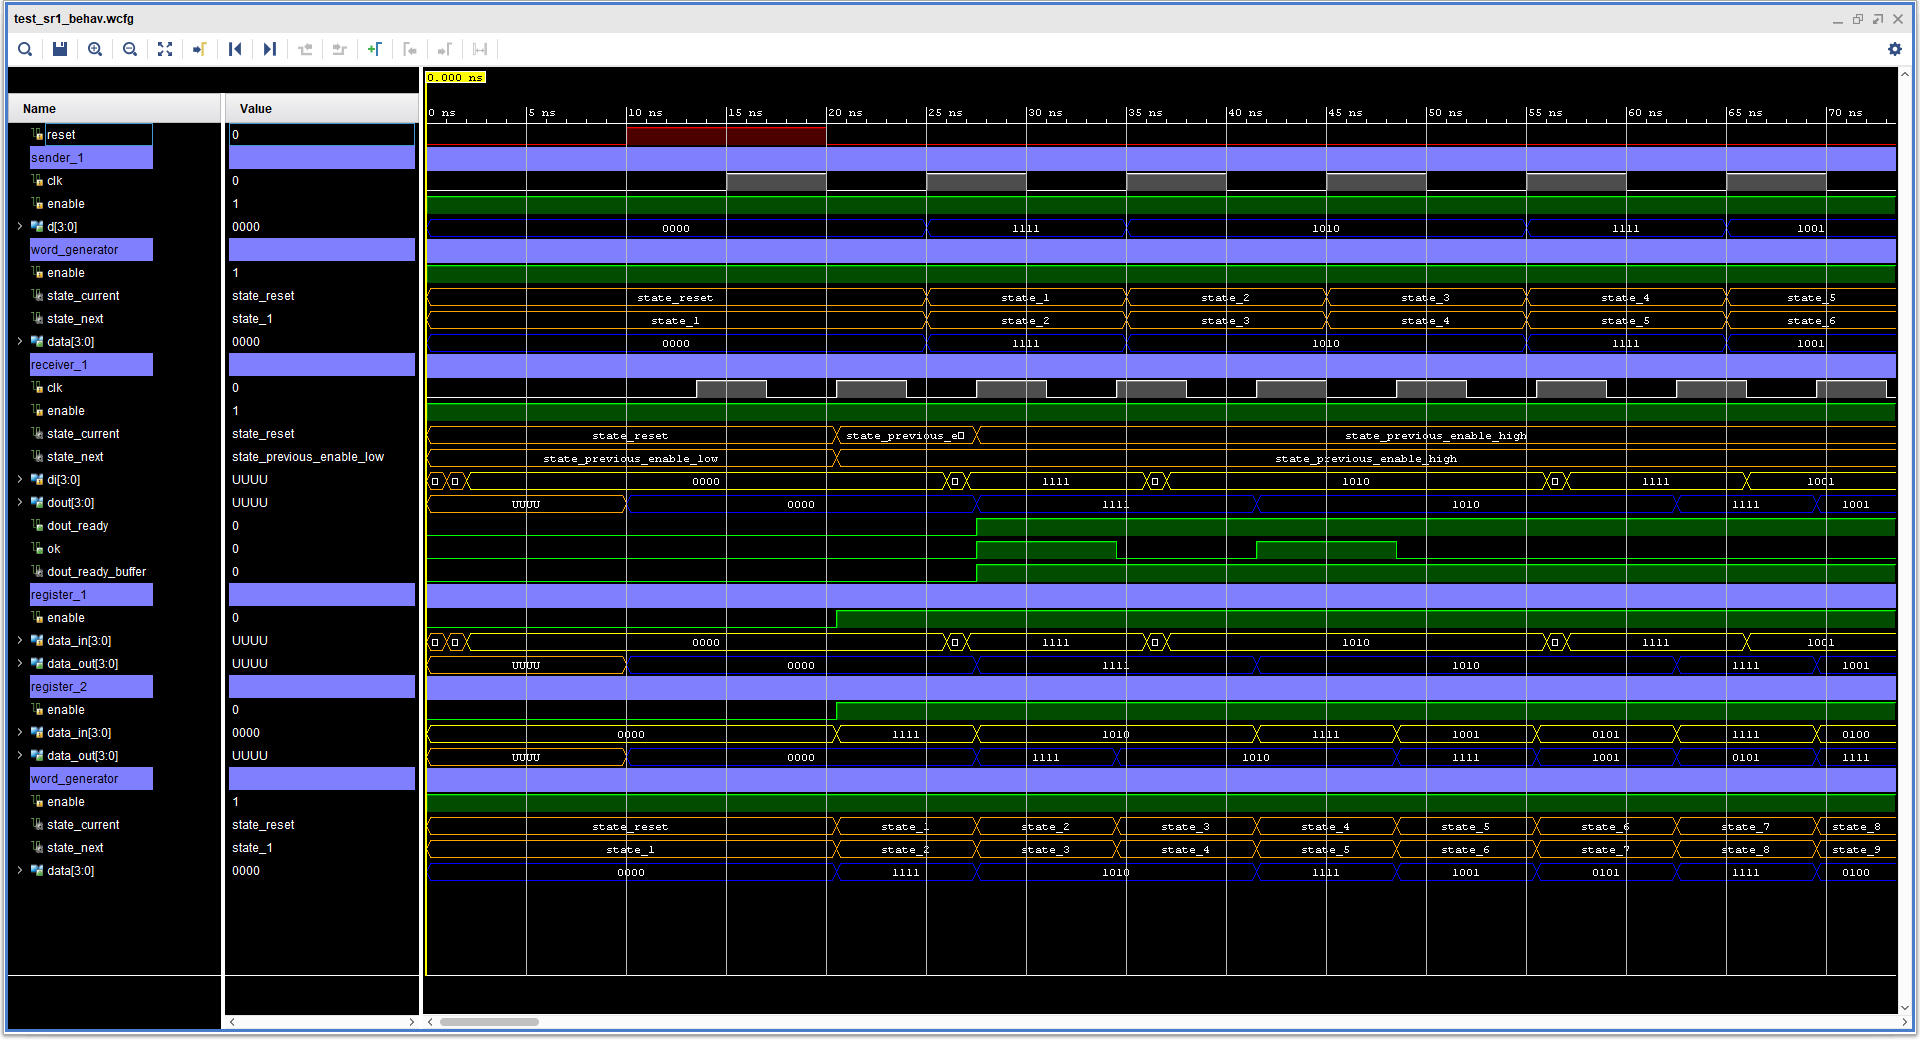
\includegraphics[trim={0 100px 0 0}, clip, width =\linewidth]{sr1_gedragssimulatie_10_7_1_2.PNG}
    \caption{\texttt{s\_1}, \texttt{r\_1} gedragssimulatie bij \(T_1 = \SI{10}{\nano\second}, T_2 = \SI{7}{\nano\second}, \Delta_1 = \SI{1}{\nano\second}, \Delta_2 = \SI{2}{\nano\second} \)}
    \label{fig:sr1_behav_10_7_1_2}
\end{figure}

\begin{figure}[htpb]
    \centering
    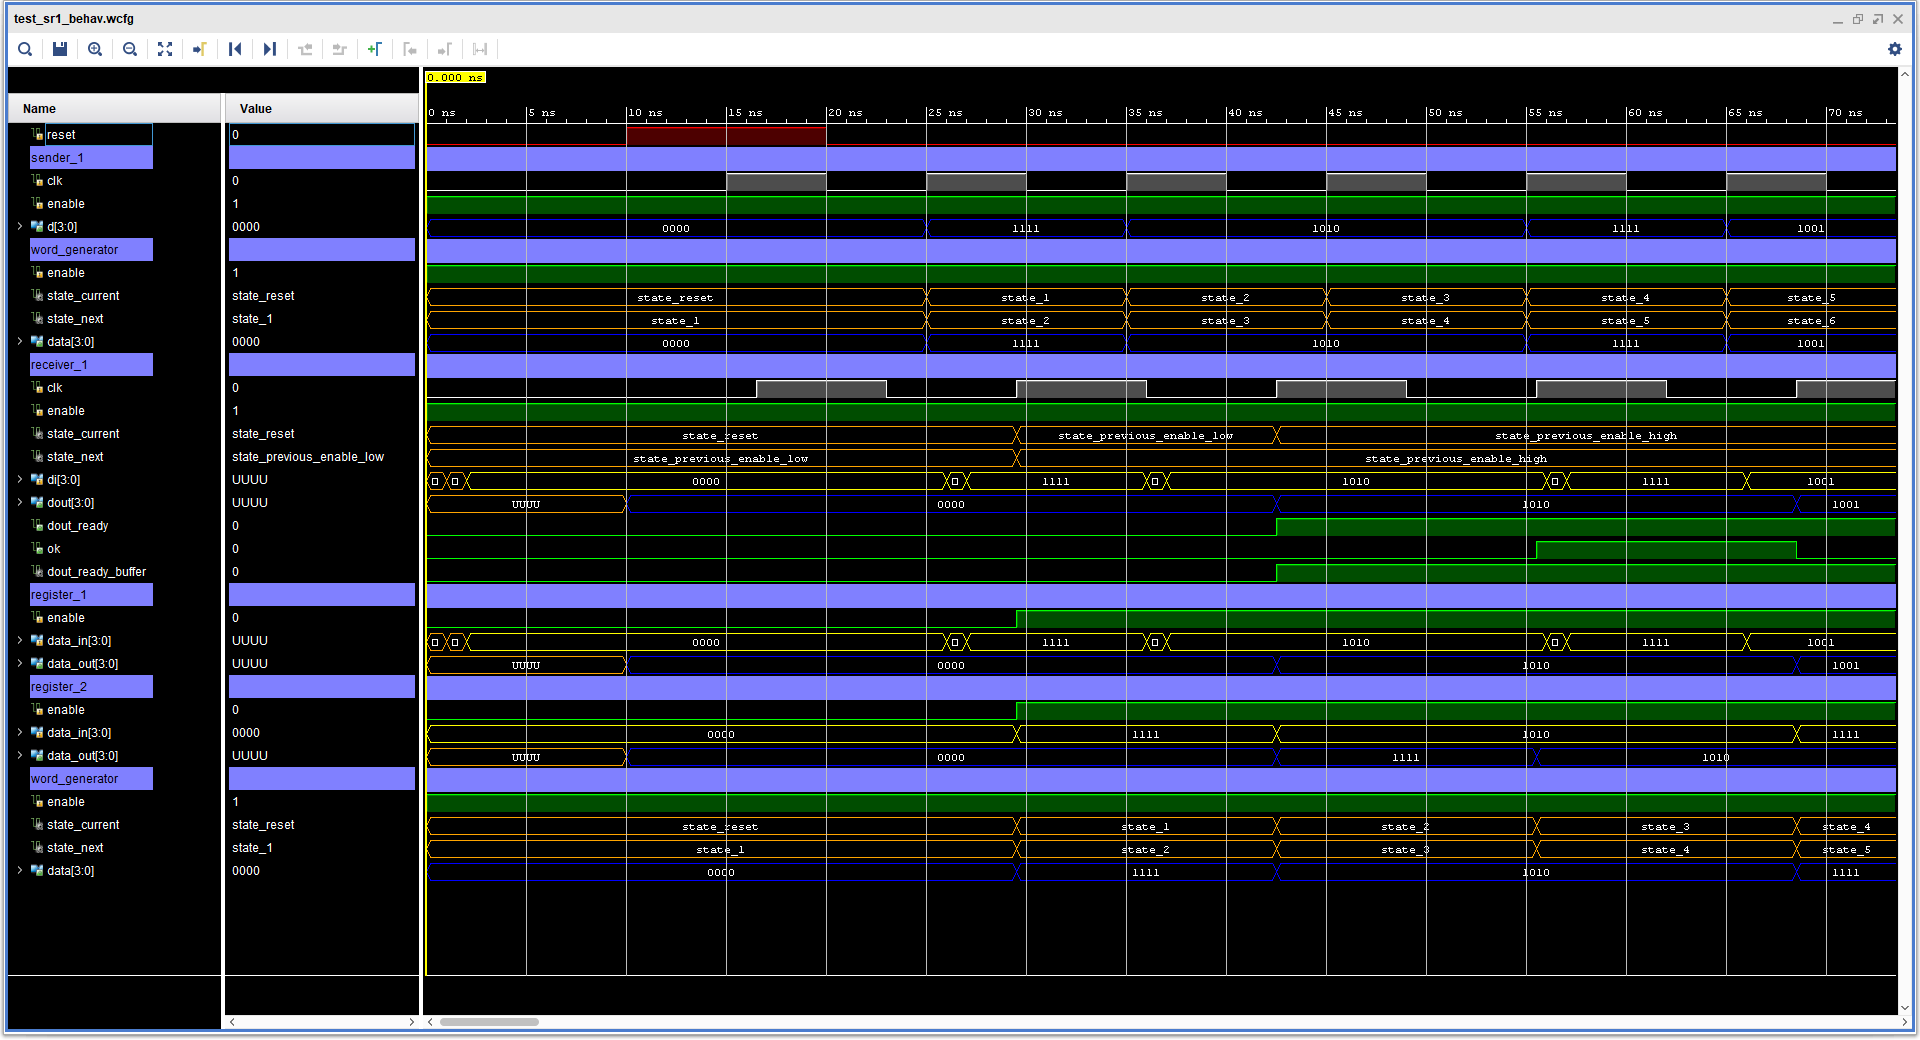
\includegraphics[trim={0 100px 0 0}, clip, width =\linewidth]{sr1_gedragssimulatie_10_13_1_2.PNG}
    \caption{\texttt{s\_1}, \texttt{r\_1} gedragssimulatie bij \(T_1 = \SI{10}{\nano\second}, T_2 = \SI{13}{\nano\second}, \Delta_1 = \SI{1}{\nano\second}, \Delta_2 = \SI{2}{\nano\second} \)}
    \label{fig:sr1_behav_10_13_1_2}
\end{figure}

\clearpage

\section{De tweede zender en ontvanger}

\begin{figure}[h!]
    \centering
    \begin{tikzpicture}
        [
        shorten >= 2 pt,
        state/.style = {
            draw, circle,
            align=center,
            minimum width = 3.5 cm,
            node distance = 4.0 cm,
        },
        ]

        % Toestanden s2
        \node[state, label = s2] (s2_wait) {\texttt{wait} \\ \texttt{(dav = '0')}};
        \node[state, below of = s2_wait] (s2_data_generation) {\texttt{data\_generation} \\ \texttt{(dav = '0')}};
        \node[state, below of = s2_data_generation] (s2_pre_data_available) {\texttt{pre\_data\_available} \\ \texttt{(dav = '0')}};
        \node[state, below of = s2_pre_data_available] (s2_data_available) {\texttt{data\_available} \\ \texttt{(dav = '1')}};
        \node[state, below of = s2_data_available] (s2_post_data_available) {\texttt{post\_data\_available} \\ \texttt{(dav = '0')}};

        % Toestanden r2
        \node[state, label = r2, right of = s2_wait, node distance = 10cm] (r2_reset) {\texttt{reset} \\ \texttt{(dreq = '0')}};
        \node[state, below of = r2_reset] (r2_wait) {\texttt{wait} \\ \texttt{(dreq = '1')}};
        \node[state, below of = r2_wait] (r2_enable) {\texttt{enable} \\ \texttt{(dreq = '1')}};
        \node[state, below of = r2_enable] (r2_timeout) {\texttt{timeout} \\ \texttt{(dreq = '0')}};


        % Transities s2
        \path
            [
            ->,
            every loop/.style = {
                in = 20,
                out = 40,
                looseness = 0
            }
            ]
            (s2_wait) edge[loop] node[right] {\texttt{dreq = '0'}} (s2_wait)
            (s2_data_available) edge [loop] node[right] {\texttt{dreq = '1'}} (s2_data_available);

        \path
            [
            ->
            ]
            (s2_wait) edge node[right] {\texttt{dreq = '1'}} (s2_data_generation)
            (s2_data_generation) edge node[right] {} (s2_pre_data_available)
            (s2_pre_data_available) edge node[right] {} (s2_data_available)
            (s2_data_available) edge node[right] {\texttt{dreq = '0'}} (s2_post_data_available)
            (s2_post_data_available) edge [bend left = 40] node[right] {} (s2_wait);

        % Transities r2
        \path
            [
            ->,
            every loop/.style = {
                in = 20,
                out = 40,
                looseness = 0
            }
            ]
            (r2_wait) edge[loop] node[right] {\texttt{dav = '0'}} (r2_wait)
            (r2_timeout) edge [loop] node[right] {\texttt{dav = '1'}} (r2_timeout);

        \path
            [
            ->
            ]
            (r2_reset) edge node[right] {} (r2_wait)
            (r2_wait) edge node[right] {\texttt{dav = '1'}} (r2_enable)
            (r2_enable) edge node[right] {} (r2_timeout)
            (r2_timeout) edge [bend left = 50] node[left] {\texttt{dav = '0'}} (r2_wait);
    \end{tikzpicture}
    \caption{\texttt{r2 en s2} toestandstransitiediagram}
    \label{fig:rs2_toestandstransitiediagram}
\end{figure}

\clearpage

\noindent \textbf{Wordt in dit protocol een veronderstelling gemaakt over de relatieve vertragingen van de signalen tussen beide automaten? Leg uit.} \\
We veronderstellen dat de vertraging op controlesignalen groter is dan de vertraging op de datasignalen.
Indien dit niet het geval is, zal de zender immers aangeven dat zijn uitgangsbits stabiel zijn, terwijl de ingangsbits van de ontvanger nog niet stabiel zijn.
Een voorbeeld van dit gedrag vinden we in figuur~\ref{fig:sr2_behav_10_12_1_50_50_2}.
Zelfs bij zeer grote vertragingen op het \texttt{DAV}-signaal blijft de communicatie tussen de automaten succesvol.
Een voorbeeld van dit gedrag vinden we in figuur~\ref{fig:sr2_behav_10_10_1_2_1_400}.
Dit wordt gegarandeerd door de 4-way handshake.

\begin{figure}[htpb]
    \centering
    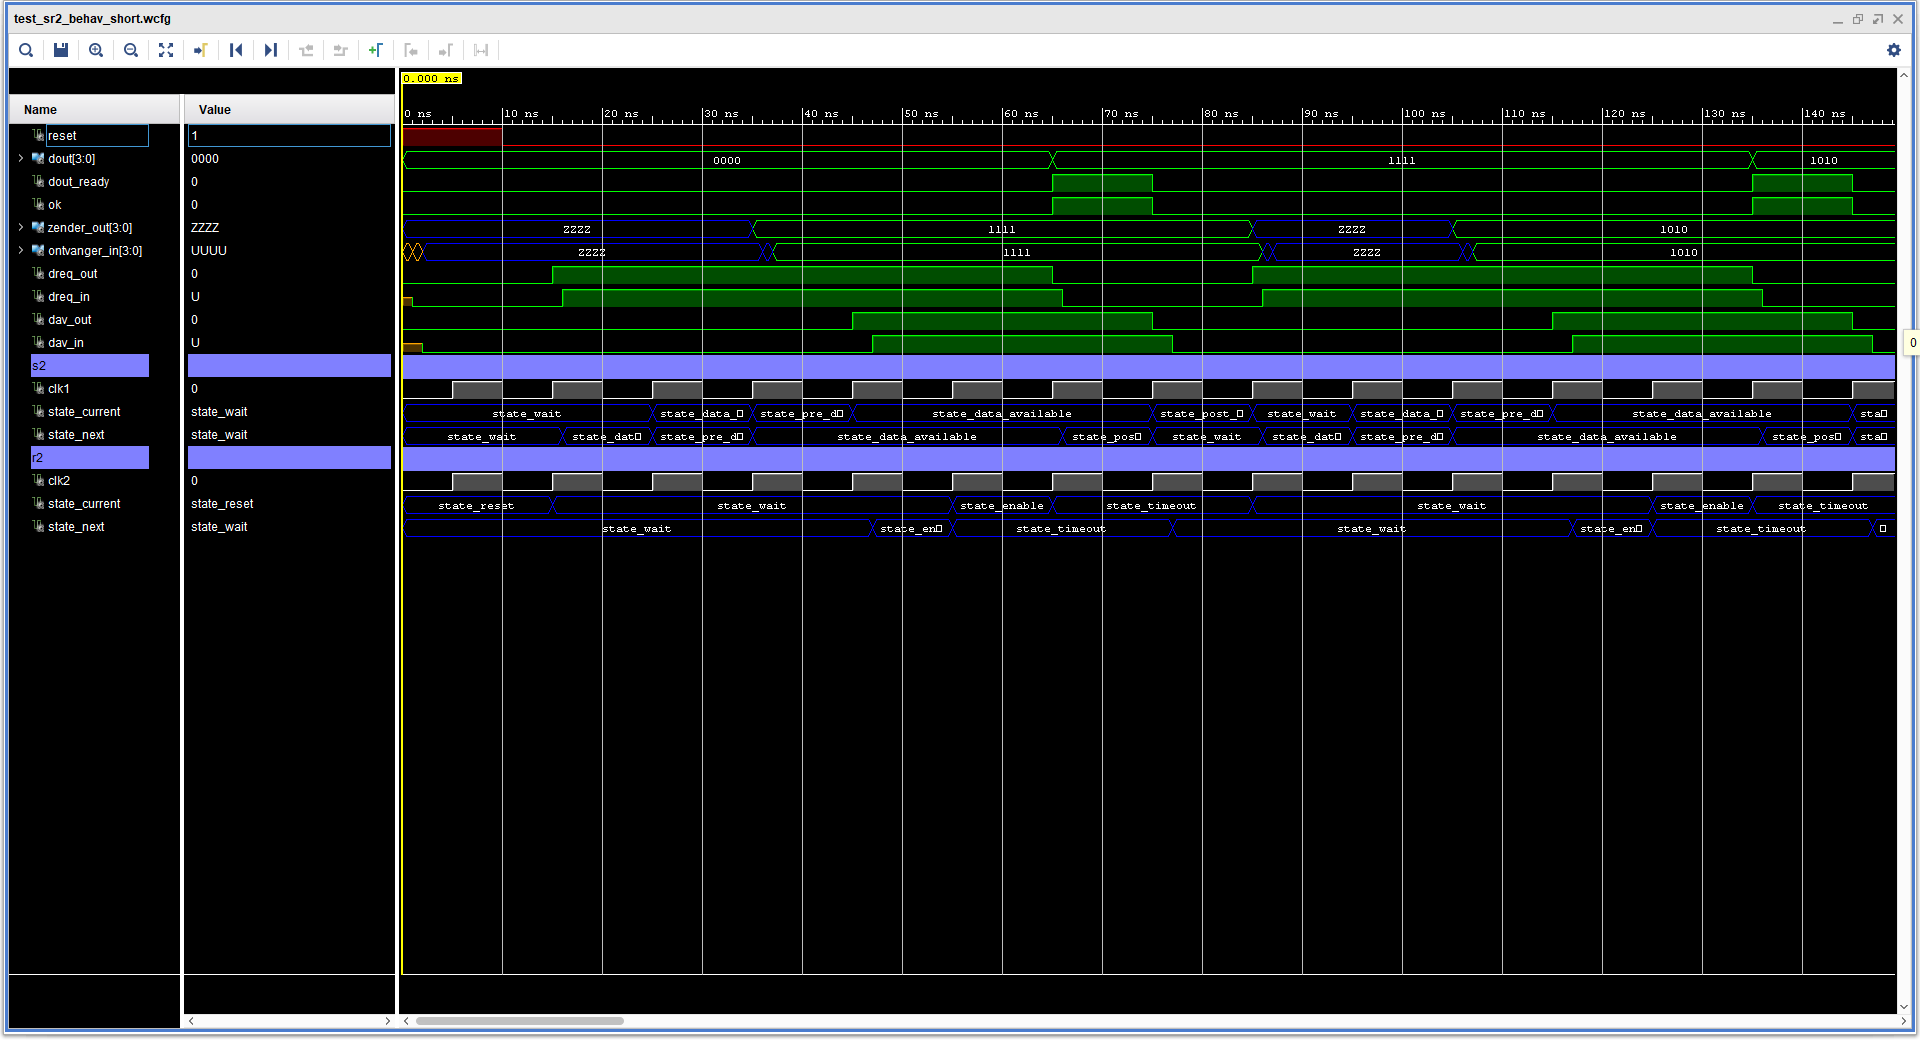
\includegraphics[trim={0 375px 0 0}, clip, width =\linewidth]{sr2_gedragssimulatie_10_10_1_2_1_2.PNG}
    \caption{\texttt{s\_2}, \texttt{r\_2} gedragssimulatie bij \(T_1 = \SI{10}{\nano\second}, T_2 = \SI{10}{\nano\second},
    \Delta_1 = \SI{1}{\nano\second}, \Delta_2 = \SI{2}{\nano\second}, \Delta_3 = \SI{1}{\nano\second}, \Delta_4 = \SI{2}{\nano\second} \)}
    \label{fig:sr2_behav_10_10_1_2_1_2}
\end{figure}

\begin{figure}[htpb]
    \centering
    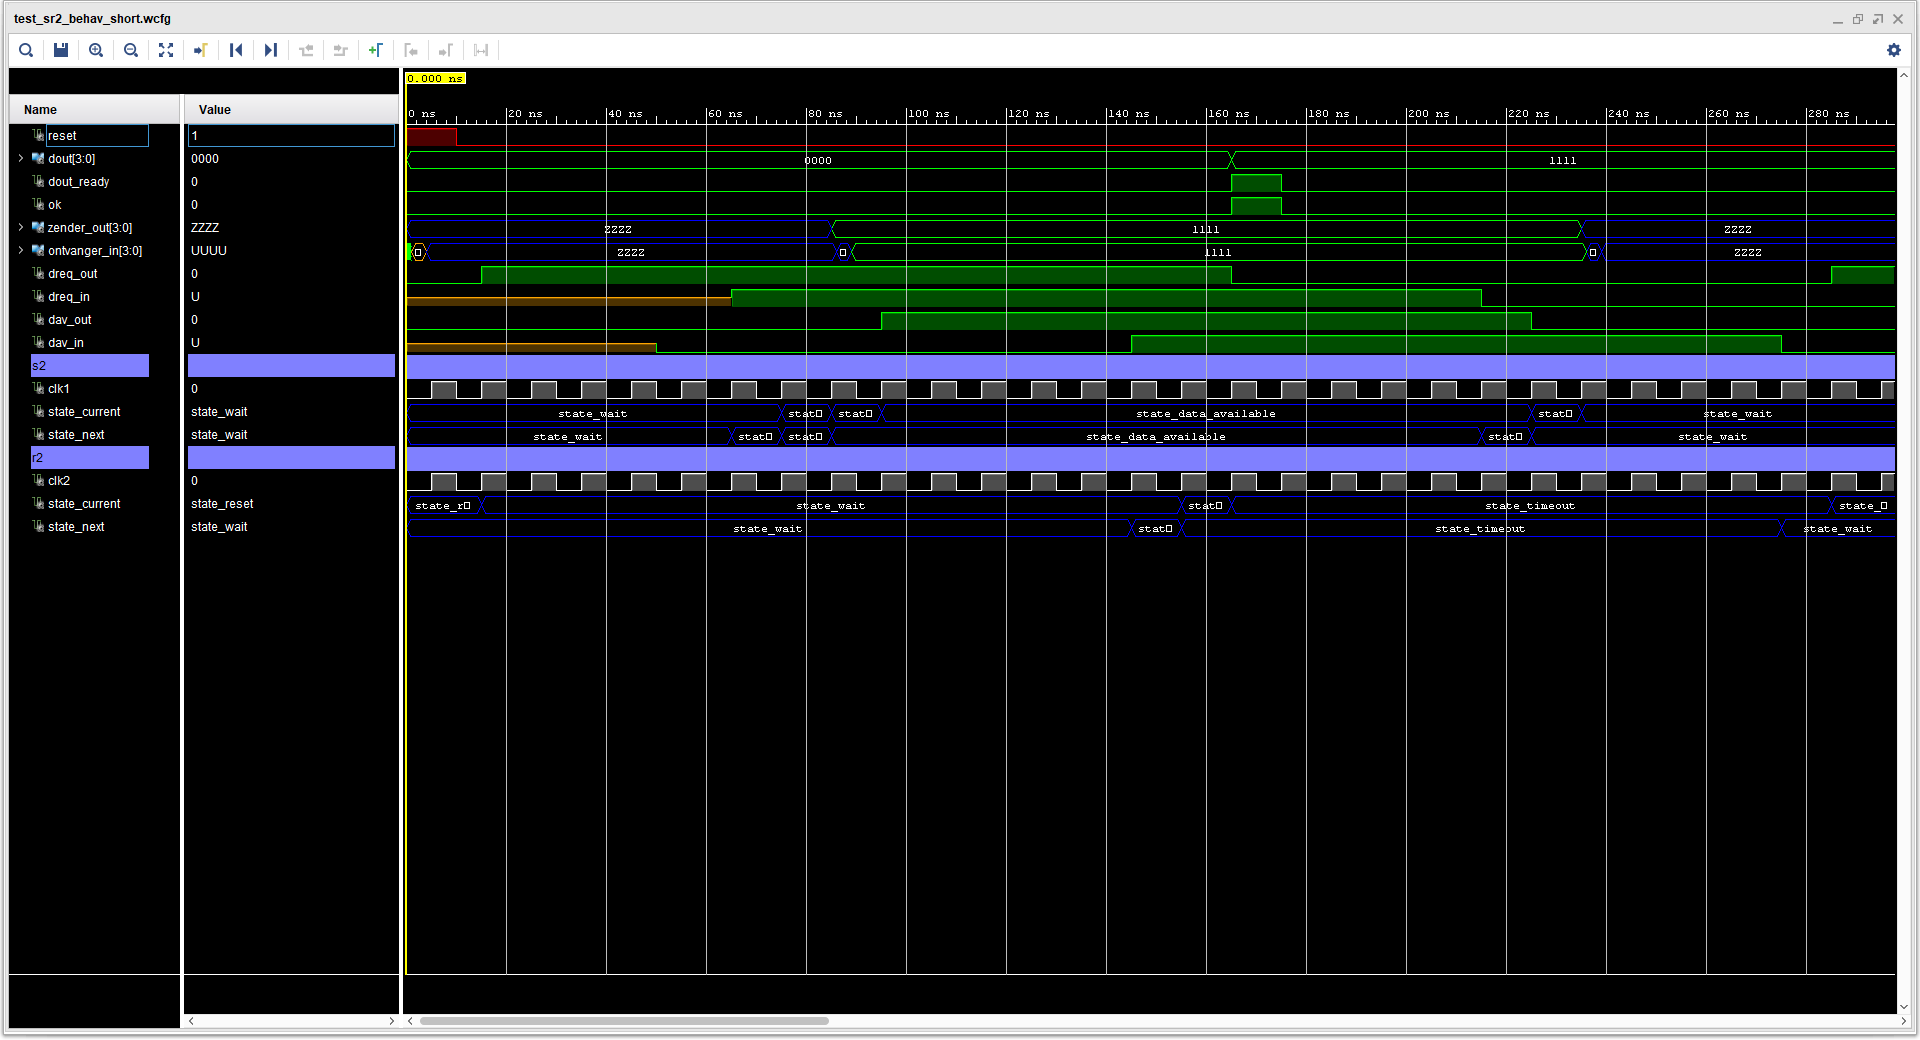
\includegraphics[trim={0 375px 0 0}, clip, width =\linewidth]{sr2_gedragssimulatie_10_10_1_4_50_50.PNG}
    \caption{\texttt{s\_2}, \texttt{r\_2} gedragssimulatie bij \(T_1 = \SI{10}{\nano\second}, T_2 = \SI{10}{\nano\second},
    \Delta_1 = \SI{1}{\nano\second}, \Delta_2 = \SI{4}{\nano\second}, \Delta_3 = \SI{50}{\nano\second}, \Delta_4 = \SI{50}{\nano\second} \)}
    \label{fig:sr2_behav_10_10_1_4_50_50}
\end{figure}

\begin{figure}[htpb]
    \centering
    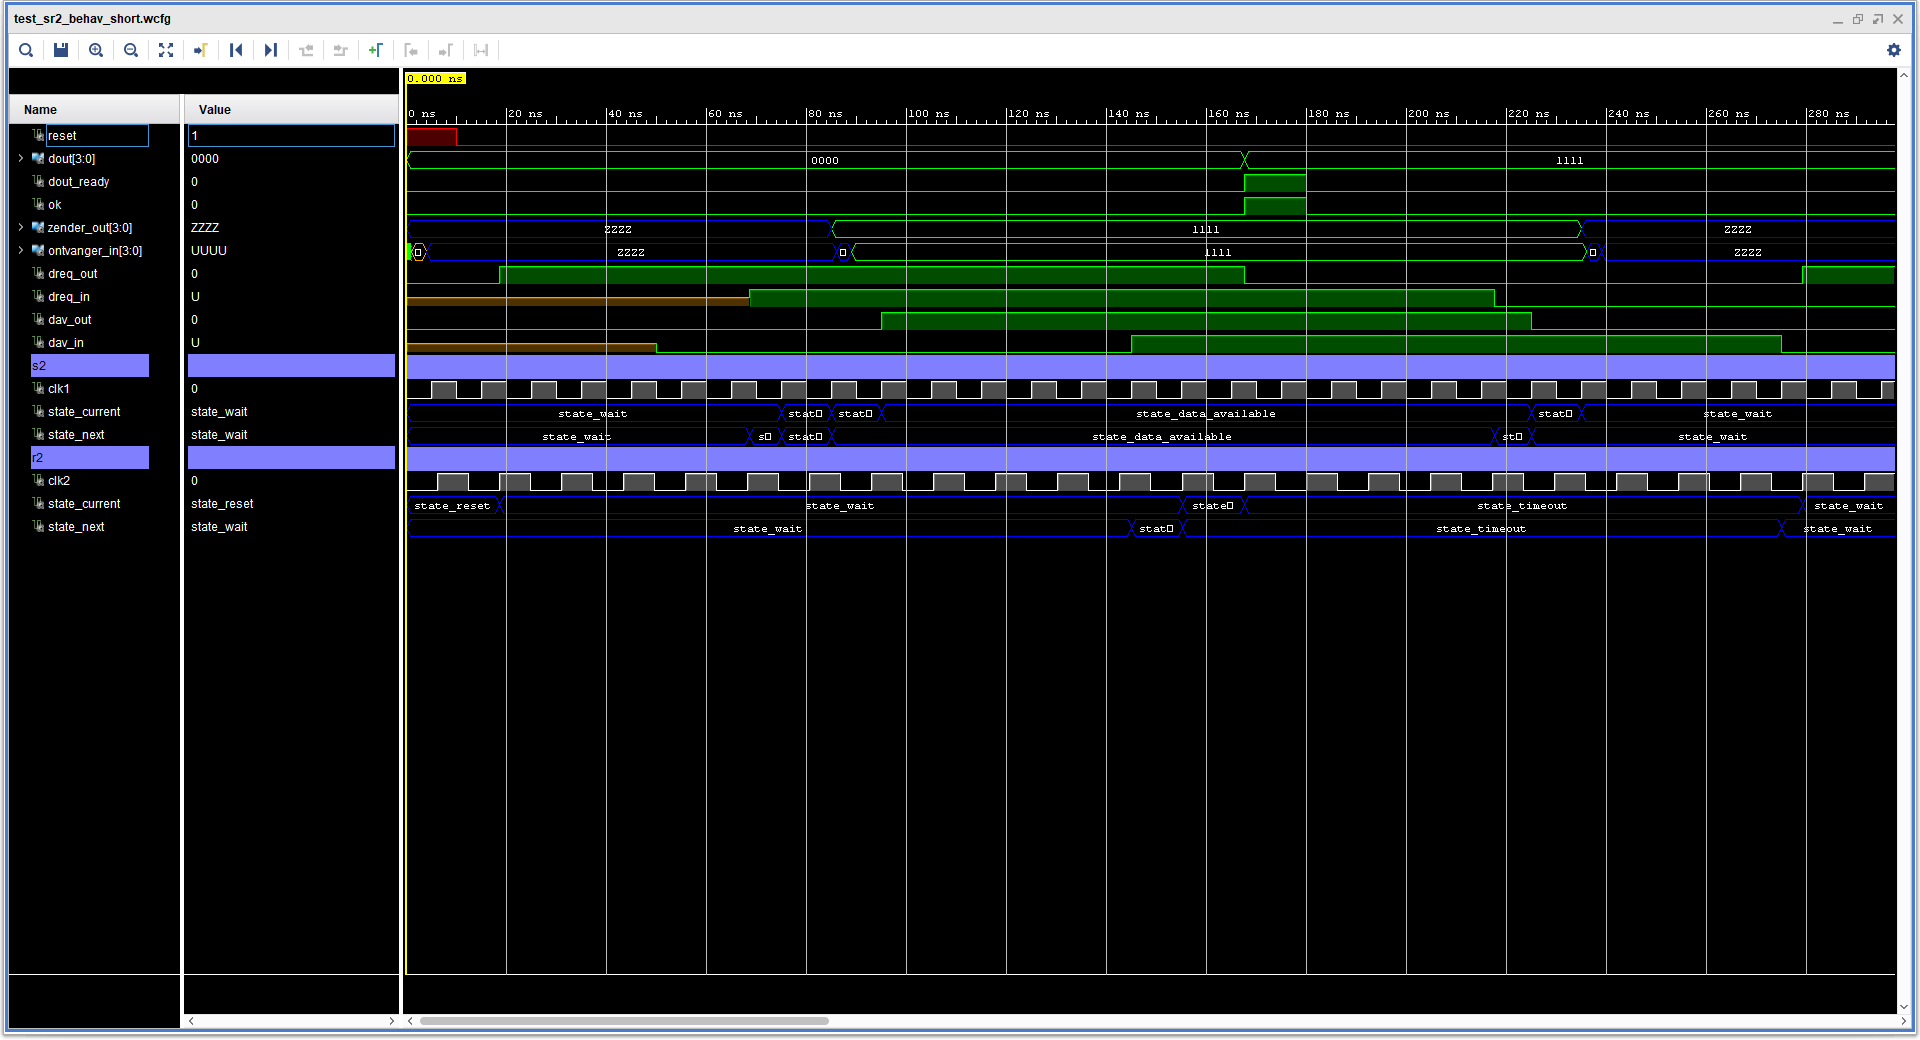
\includegraphics[trim={0 375px 0 0}, clip, width =\linewidth]{sr2_gedragssimulatie_10_12_1_4_50_50.PNG}
    \caption{\texttt{s\_2}, \texttt{r\_2} gedragssimulatie bij \(T_1 = \SI{10}{\nano\second}, T_2 = \SI{12.4163}{\nano\second},
    \Delta_1 = \SI{1}{\nano\second}, \Delta_2 = \SI{4}{\nano\second}, \Delta_3 = \SI{50}{\nano\second}, \Delta_4 = \SI{50}{\nano\second} \)}
    \label{fig:sr2_behav_10_12_1_4_50_50}
\end{figure}

\begin{figure}[htpb]
    \centering
    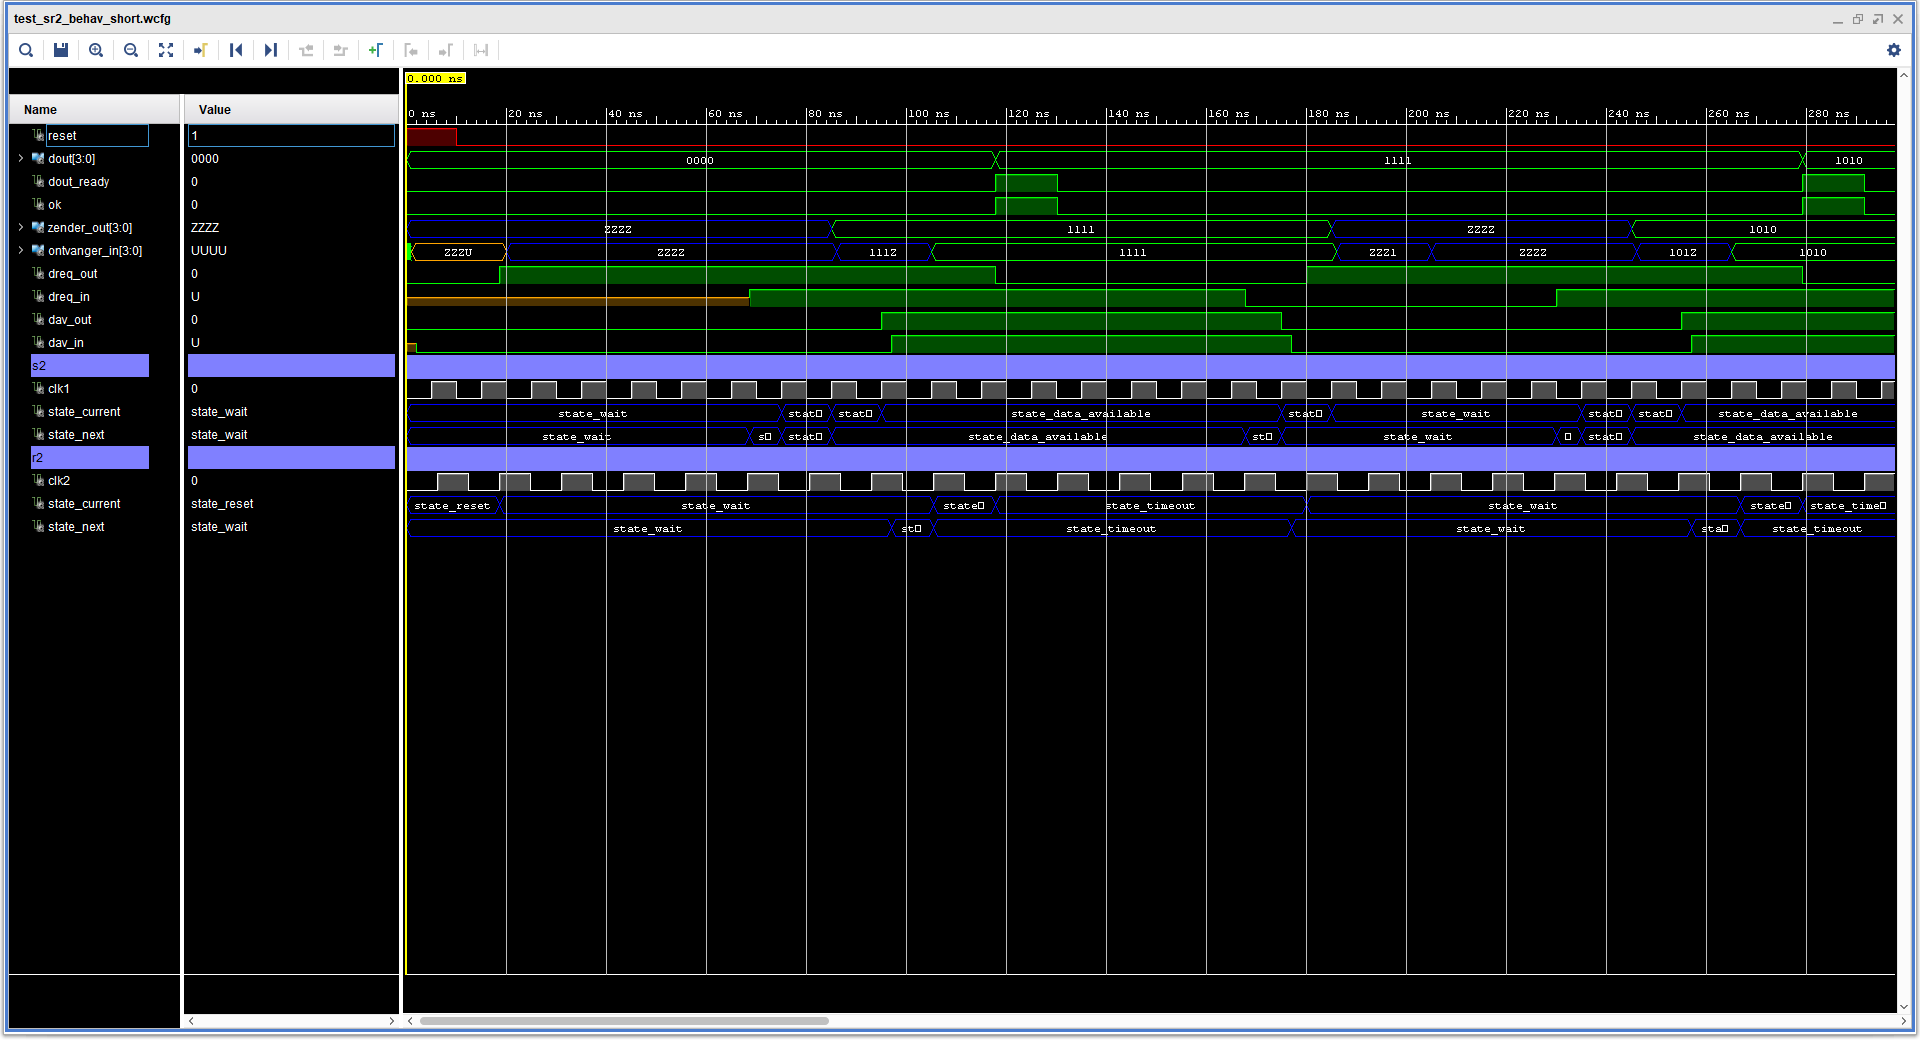
\includegraphics[trim={0 375px 0 0}, clip, width =\linewidth]{sr2_gedragssimulatie_10_12_1_20_50_2.PNG}
    \caption{\texttt{s\_2}, \texttt{r\_2} gedragssimulatie bij \(T_1 = \SI{10}{\nano\second}, T_2 = \SI{12.4163}{\nano\second},
    \Delta_1 = \SI{1}{\nano\second}, \Delta_2 = \SI{20}{\nano\second}, \Delta_3 = \SI{50}{\nano\second}, \Delta_4 = \SI{2}{\nano\second} \)}
    \label{fig:sr2_behav_10_12_1_20_50_2}
\end{figure}

\begin{figure}[htpb]
    \centering
    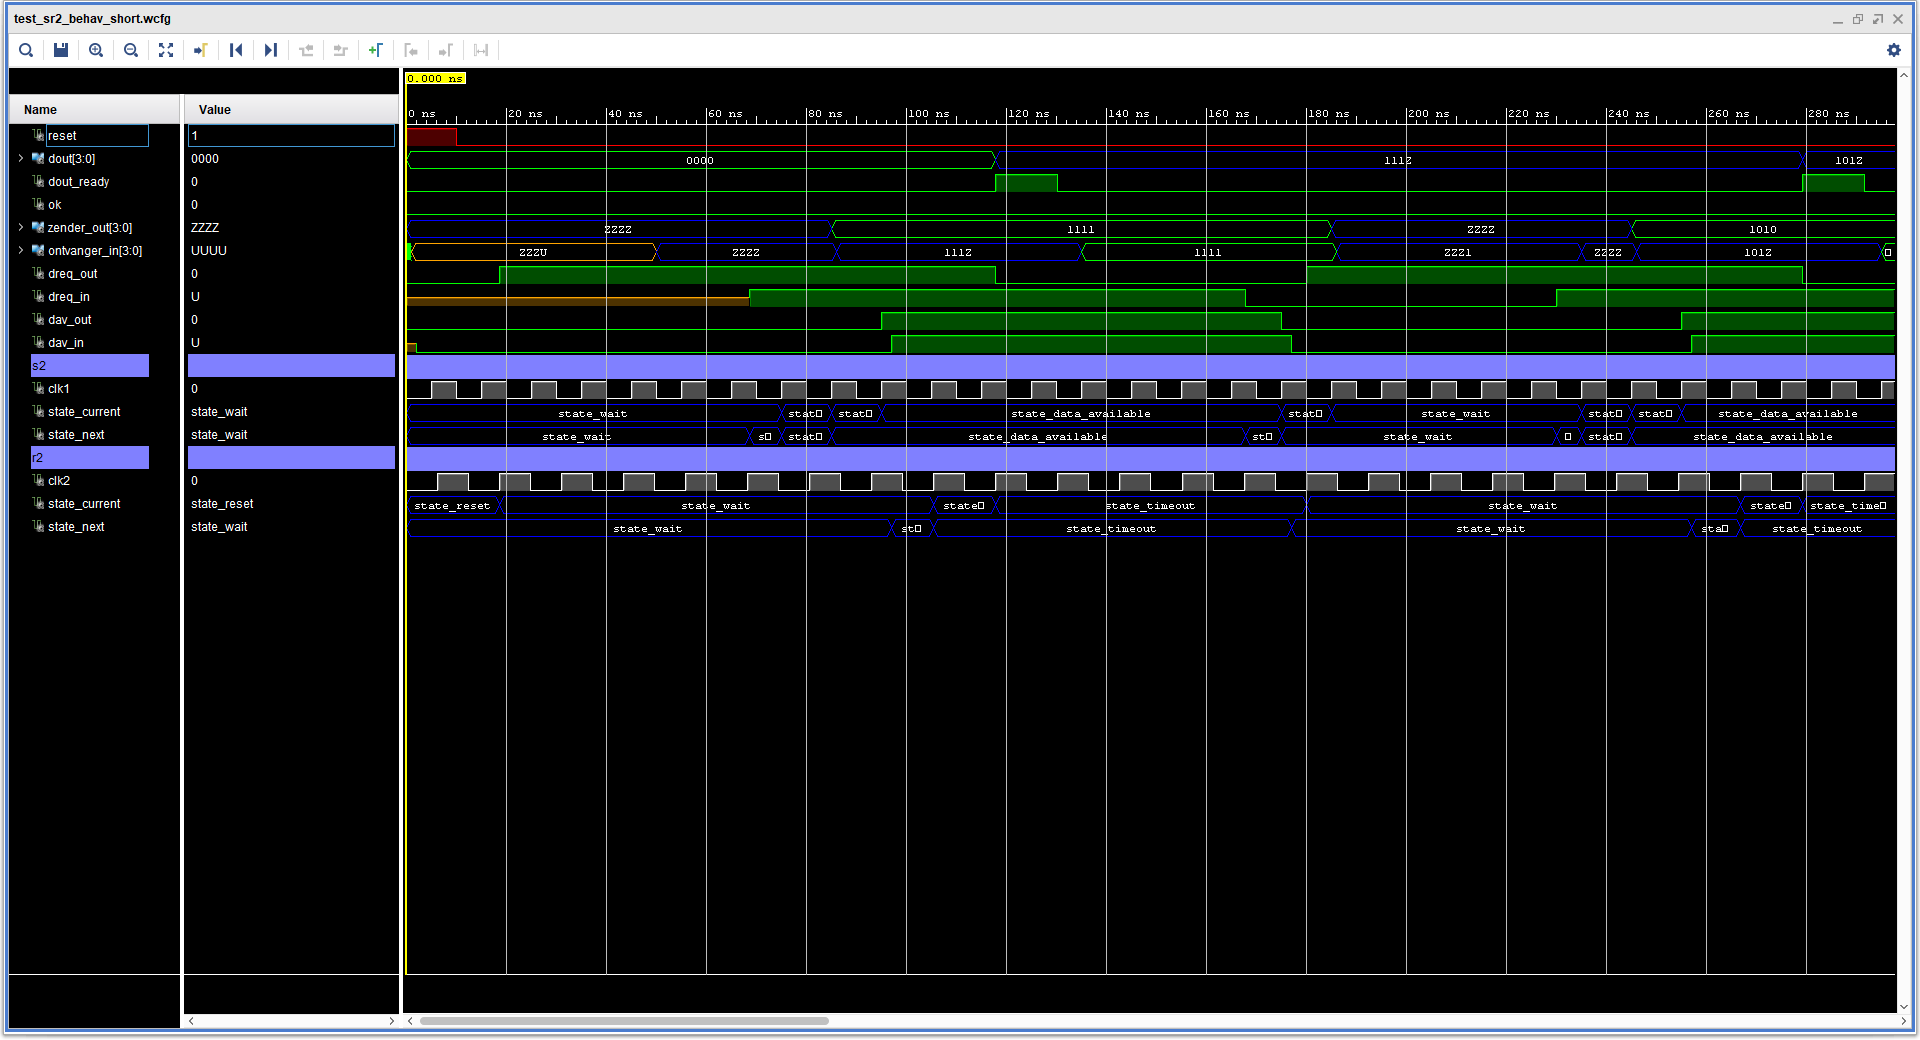
\includegraphics[trim={0 375px 0 0}, clip, width =\linewidth]{sr2_gedragssimulatie_10_12_1_50_50_2.PNG}
    \caption{\texttt{s\_2}, \texttt{r\_2} gedragssimulatie bij \(T_1 = \SI{10}{\nano\second}, T_2 = \SI{12.4163}{\nano\second},
    \Delta_1 = \SI{1}{\nano\second}, \Delta_2 = \SI{50}{\nano\second}, \Delta_3 = \SI{50}{\nano\second}, \Delta_4 = \SI{2}{\nano\second} \)}
    \label{fig:sr2_behav_10_12_1_50_50_2}
\end{figure}

\begin{figure}[htpb]
    \centering
    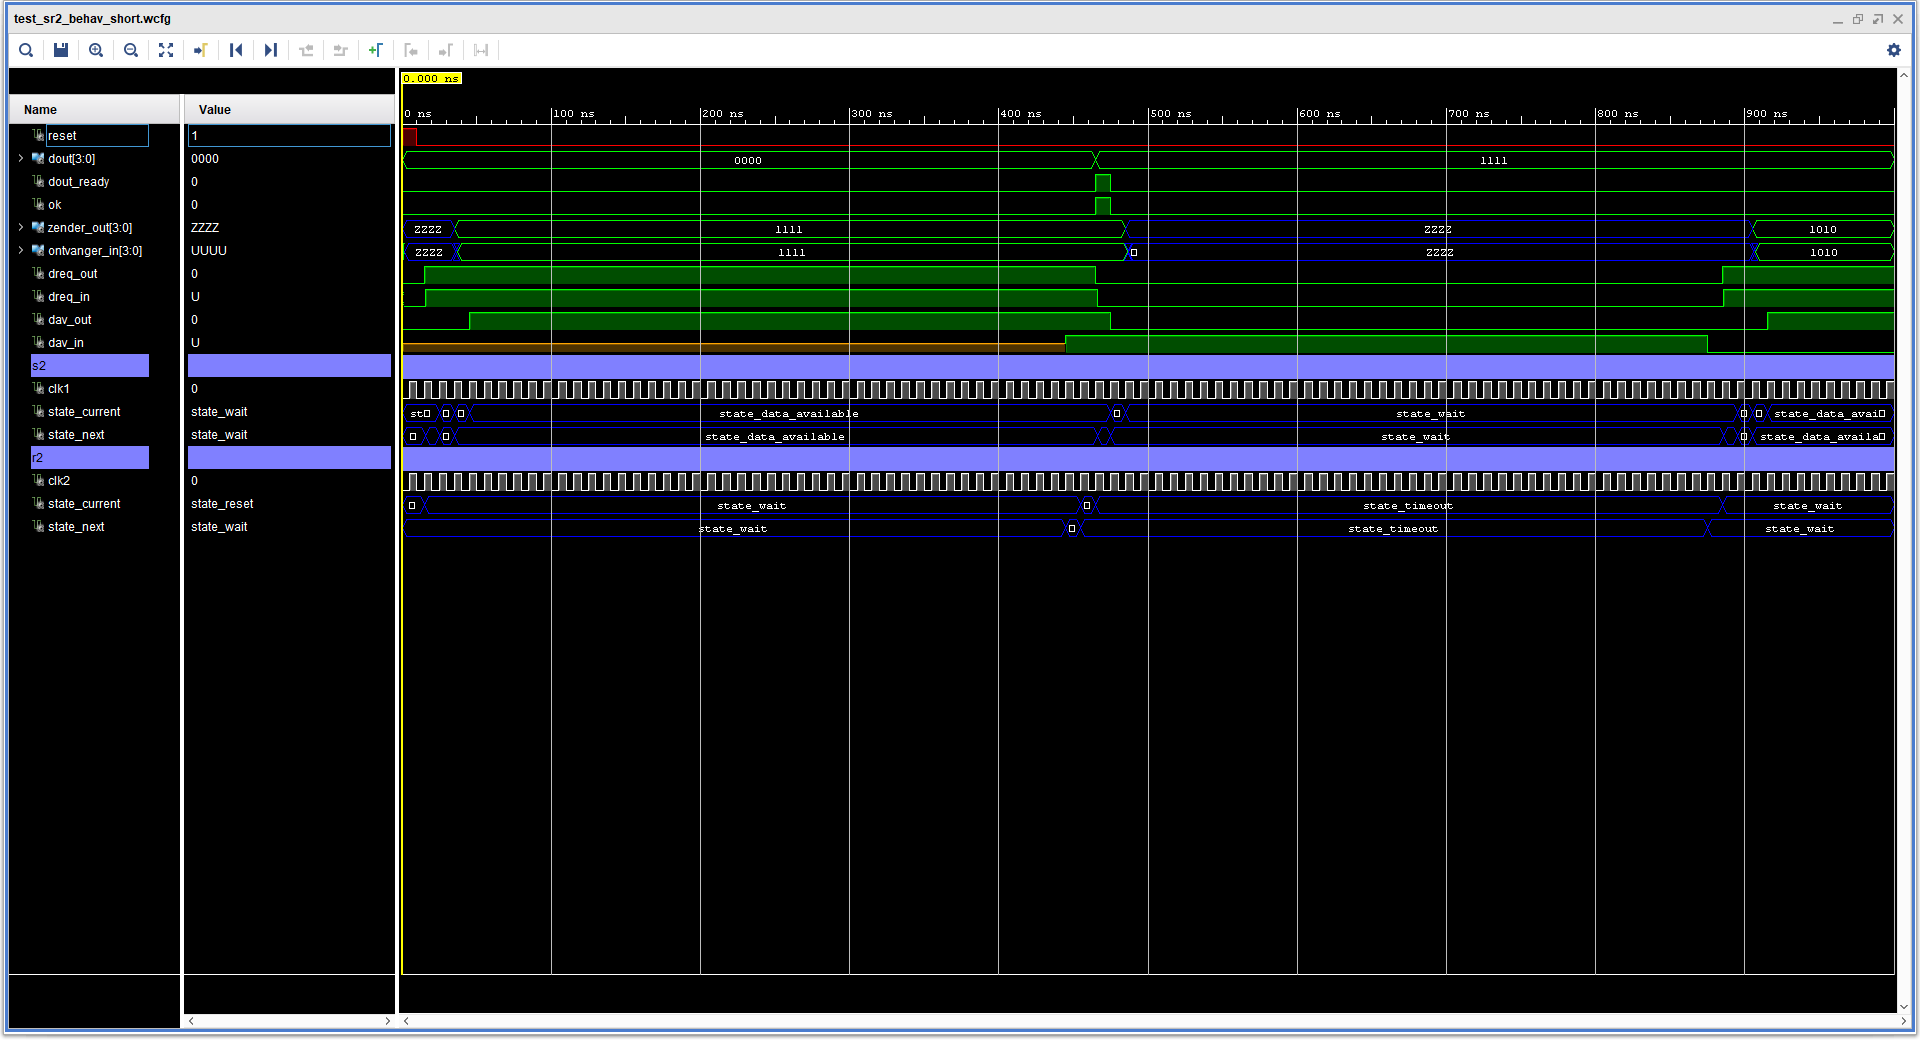
\includegraphics[trim={0 375px 0 0}, clip, width =\linewidth]{sr2_gedragssimulatie_10_10_1_2_1_400.PNG}
    \caption{\texttt{s\_2}, \texttt{r\_2} gedragssimulatie bij \(T_1 = \SI{10}{\nano\second}, T_2 = \SI{10}{\nano\second},
    \Delta_1 = \SI{1}{\nano\second}, \Delta_2 = \SI{2}{\nano\second}, \Delta_3 = \SI{1}{\nano\second}, \Delta_4 = \SI{400}{\nano\second} \)}
    \label{fig:sr2_behav_10_10_1_2_1_400}
\end{figure}

\clearpage

\section{Synchronisatieflipflop}

\noindent \textbf{Bedenk voor welke toestandsassignatie dit bij jullie ontvanger-automaat voor problemen kan zorgen. Leg duidelijke uit wat er fout loopt aan de hand van een schets van simulatiegolfvormen (ontvangerklok, DAV en de individuele toestandsbits van de ontvangerautomaat) waarin de volgorde van de gebeurtenissen en de vertragingen zo zijn gekozen dat het fout loopt. Toon ook aan voor dezelfde situatie hoe een synchronisatieflipflop	het probleem oplost.}

In r2 kunnen er zich 2 kritische races voordoen bij een toestandstransitie.
Bij een overgang van state_enable naar state_reset en van state_timeout naar state_wait moeten er 2 toestandsbits aangepast worden,
de volgorde waarin dit gebeurt is hierbij van belang aangezien de mogelijke tussentoestanden telkens stabiel zijn.
Door te synchroniseren met een synchronisatieflipflop (Hamming-afstand 1) zullen de toestandsbits al meer dan 1 klokcyclus stabiel zijn.

\end{document}

